% !TEX encoding = UTF-8 Unicode

\documentclass[12pt]{ltjsarticle}

\usepackage{graphicx}
\usepackage[deluxe]{luatexja-preset}
\usepackage{luatexja-otf}
\usepackage{url}
%\usepackage{kougai}

\title{少子化によるVRデートアプリの提案について}
\author{1932158 小池 周平  指導教員 中村 直人 教授}

\begin{document}

\maketitle

\section{はじめに}


%背景

2015年9月に150カ国を超える世界のリーダーが参加して開かれた「国連持続可能な開発サミット」でSDGsと呼ばれる「持続可能な開発目標」が掲げられた.このSDGsの中に近年,日本で大きな問題となっている少子化も含まれている.
少子化は,解決するのが遅れれば遅れていくほど悪化し,早急に解決しなくてはならない問題であり,この要因は,晩婚化の進展,交際率・婚姻率の減少などとされている.

% 要因を上の業で定義しているので,次にこれらの要因について,順番にもう少し詳しく述べていく必要あり

%全体の要因
%現在少子化は,様々な問題点が存在している.  % 少子化の問題点=労働人口減少や人口ピラミッド逆転などなので,ちょっと言葉が違います.
 % https://www.ipss.go.jp/ps-doukou/j/doukou15/doukou15_gaiyo.asphttps://www.ipss.go.jp/ps-doukou/j/doukou15/doukou15_gaiyo.asp
% 晩婚化の進展について
% 書いてね
近年では女性の社会進出により男女間の格差がなくなり,以前よりも結婚するより仕事に時間を費やしたいと思う女性が増えているため晩婚化が進んでいると考えられる\cite{sasaki2012}.

% 交際率・婚姻率の減少について
% 主観は不要なので事実のみを書く(ここで言う主観=〜と思い調査した など)
一方,18〜34歳の結婚意欲の調査結果によると,1987年〜2010年の結婚意欲はほとんど変化していない.
すなわち,「結婚はしたいけれど,良い相手に恵まれない」と思っている率が高いこととなる\cite{naikakufu2019}.
これは,「出会いの場の減少」と「交際への不安」と言い換えることができる.

% 問題点と目的
よって,出会ってからデートに進展するまでをサポートできれば,婚姻率上昇に繋げられるのではないかと考えた.
ここで,SNSやマッチングアプリを通じて出会うことに抵抗を感じる人が多いことが問題となる.
そこで本研究では,VRデートアプリを提案し,将来的な婚姻率上昇に繋がる意識改革の可能性について調査を行うことを目的とする.

\section{問題の原点}
%コメント読んでね.
% 通常,1章には図や表を使わないので,2章でそれらを補足する.
% 晩婚化や結婚意欲などについて,図を用いて再度説明する.(そのために1章ではほとんど説明しないように修正した)
% 気をつけることは,主観で書かずにデータで攻めることである.
% ここで,どこまでデータで攻めつつ,自分の研究に誘導するかが醍醐味である.
% 今回は,晩婚化が進んでいることや,結婚意欲が変わっていないことなどを説明しつつ,マッチングアプリやSNSの話を通じて,いきなり会うのは怖いよねというところに着地できればOK.
% データは,これまでに参照したものに加えて,下記からも参照すること.
% https://www.ipss.go.jp/ps-doukou/j/doukou15/doukou15_gaiyo.asp
晩婚化について表\ref{table:shokon}にあるように平成7年から平成27年にかけての20年間で平均初婚年齢が夫は2.6歳,妻は3.1歳増加している.
ここで,晩婚化は何が引き起こしているのかを考える.
図\ref{fig:dokusin}が示しているように男女ともに結婚できない理由として一番多いのが「適当な相手に巡り合えない」である\cite{doukou}.
つまり,「適当な相手に巡り合えれば結婚をしたい」ということになる.
また結婚しない理由として「趣味や娯楽を楽しみたい」や「仕事(学業)にうちこみたい」など時間をとることが出来ないというものもある\cite{doukou}.
加えて結婚意欲に関しては図\ref{fig:教科書}のように18~34歳の結婚意欲は23年間で男女それぞれ5.5\%と3.5\%程度しか減少していない.
よって,結婚意欲はほとんど減少していないことが分かる.
また,現在交際している男女181名にどのようにして異性と知り合ったのかのアンケートをとったところ,一番が「幼稚園から大学までの知り合い」という結果に次いで「アプリを利用して知り合った」という回答が得られた\cite{cancan}.
学生から社会人になってしまうと趣味嗜好の合う相手と会うのが難しくなってくる.
ここから,多くの社会人が利用するのがマッチングアプリである.
一方,マッチングアプリ自体に懸念を抱いている方は多く,マッチングアプリに関する印象アンケートでは「詐欺や宗教勧誘にあいそう」,「犯罪にあいそう」などの回答が得られた\cite{prtimes}.
%一方,結婚意欲に関しては図\ref{fig:教科書}のように18\~34歳の結婚意欲は1987年の男性が91.8\%,女性が92.9\%に対し2010年の男性が86.3\%,女性が89.4\%と23年間でそれぞれ5.5\%と3.5\%程度しか減少していない.
\begin{table}
\centering
  \caption{平均初婚年齢}
  \label{table:shokon}
  \begin{tabular}{rrr}
   & 夫(歳) & 妻(歳) \\
  平成7年 & 28.5 & 26.3 \\
  平成17年 & 29.8 & 28.0 \\
  平成23年 & 30.7 & 29.0 \\
  平成24年 & 30.8 & 29.2 \\
  平成25年 & 30.9 & 29.3 \\
  平成26年 & 31.1 & 29.4 \\
  平成27年 & 31.1 & 29.4 \\
  \end{tabular}
  \end{table}
\begin{figure}[h]
\centering
 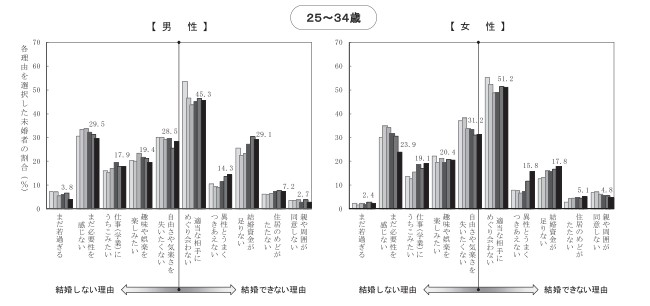
\includegraphics[width=170mm]{bannkonnriyuu.jpg}
 \caption{25~34歳の男女が独身にとどまっている理由の選択割合}
 \label{fig:dokusin}
\end{figure}
%目的


%ほどが減少していることから未婚者が結婚意欲をそがれているのではないかと思い調査したが図\ref{fig:教科書}にあるように男性・女性ともに85%がいずれは結婚したいと答えており意欲が大きく下がっているわけではないと確認できた\cite{naikakufu2019} .
%次に交際率,婚姻率の減少がどこからきているのかについて考える.その理由として交際への不安というものが取り上げられる.
%さらに交際への不安がどこからきているのかを考えると出会いの場が少ないという点と時間がないという二つがあげあれる.
%出会いの場自体の例を挙げるとすると,学校や職場,サークルや部活,友人づての紹介,マッチングアプリなどが挙げられる.この中で学校,職場,サークル,部活は出会った相手が自分の趣味や嗜好と会うかはわからず,出会いを目的としている人からすると自分と合う人物と巡り合える確率は低いと思われる.

% 公平に見て,学校(サークルや部活)は,活動内容に興味がある人が集まるので,自分と合う人物と巡り会える確率は高いほうです.
% むしろ参照内容はどこに書いてありました?


%学校や職場などで出会った人と仮に交際まで行けたとしてもその後折り合いが合わなくなり別れることになったとき,別れた後でも顔を合わせる機会があることから付き合うこと自体がリスクにもなりうる.
%それらのことから出会いを求めているのであれば相手の嗜好が出会う前から知ることができ,別れたあとのリスクを負うことのないマッチングアプリが最も適しているかと考えられる.
%しかし,現在存在しているマッチングアプリのイメージはあまり良いものではなく真剣に交際を考えていて,これから初めてマッチングアプリを利用する者にとっては不安が大きいのではと考えた\cite{yoshimura2020}.
%また,出会いの場が減少していることからデート未経験者にとってデートというものに大きな壁を感じ交際の第一歩を踏み出せないということもあるかとも考えられる.

% 必要な流れはコメントに書きました.
% 学校や職場で相手を見つけた
% YES -> デートに誘いたいがプランがわからない,会うのが怖い
% NO -> マッチングアプリやSNS -> 会うのが怖い
% SNSで文字ベースのやり取り -> 会わないと実態がわからない -> 会うのが怖い
% Web会議 -> 身バレ怖い,時間がない
% VRChat -> 時間がない
% 会うのが怖い,身バレが怖いの改善策 -> VR上で会うことで改善
% 時間がないの改善策 -> VR内で時間を決めて会うことで改善
% 会わないと実感がわかないの改善策 -> VR内で共通体験してその後お喋りをすることで改善

仮に学校や職場,マッチングアプリで合いそうな人を見つけたとしても二人きりで直接会うことに恐怖を感じるという方は多く存在する\cite{yoshimura2020}.また,既に付き合っていても時間がない為にデートをすることが出来ないという人も存在する.
そこで,これらを全て解決し交際について前向きになる方法を探っていく.
初めて会うのが怖いというものは電話やWeb会議,VRなどを駆使すれば解決するかと思われる
デートが初めてでどういったようにすればいいか分からないという方には何かしらのシステムで行く場所の指定をすれば外すリスクは少ないのではないかと思われる.
一度会ってから合うか合わないかの確認,時間がない等も仮想的な空間で短時間で体験できるシステムであれば解決するだろうと考えられる.
これらの解決策から私はVRデートアプリケーションというものを提案する.
\begin{figure}[h]
\centering
 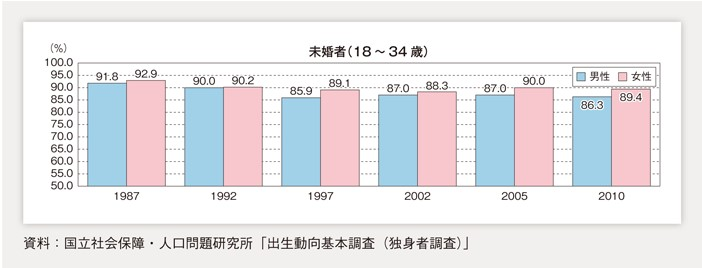
\includegraphics[width=150mm]{iyoku.jpg}
 \caption{いずれ結婚したいと思っている18歳~34歳の未婚者の割合}
 \label{fig:教科書}
\end{figure}
%目的

\section{VRデートアプリについて}
前節で説明したように,VR空間内でデートするアプリを開発すれば,少子化の改善に寄与できると考えられる.
そこで,個別の問題点を以下のように改善する方法を考案する.
まず,会うのが怖い,身元がばれることが怖いについては,VR空間内で擬似的にデートを行うことで改善できる.
% 身バレは使わないほうが良い表現なので,適当に変えてください.
次に,時間がないことに対しては,デートの時間を40分〜1時間に設定し,仕事帰りのちょっとした時間でも体験できるようにすることで改善できる.
また,会わないと実感がわかないことに対しては,デート時間の前半に共通の体験をしてもらい,後半はその体験についておしゃべりする時間としてお互いの性格を知る機会を設けることで改善できる.
本研究では,以上のコンセプトから,VRデートアプリの仕様を定めている最中である.

現在考えている仕様は以下のようなものであり,画面構成は図\ref{fig:イラスト}のようなものを想定している.
アプリケーションの実装は,Unityを使用することを考えている.

\begin{itemize}
\item デート会場:水族館,港
\item 所要時間:体験とおしゃべり併せて40〜60分
\item デートの進行:時間が限られているので,自動進行するアトラクション型
\item その他:表情や手の動きをキャプチャして,共感や共通体験を可能にする
\end{itemize}
% 表でもOK,文章でもOK




%このアプリケーションはまだデートをしたことがない方,初対面で会うのが怖いと思っている方に向けたアプリケーションである.
%アバターは自分の容姿と似ているものを用意し,VR空間を利用して疑似的なデートをするというものである.
%仮想的な場所でありながらお互いを認知することができ,場所はシステム側で設定し,40分から1時間程度という短い時間でデートをすることが可能である.

%アプリケーションの実装において必要なものは
%・上記で挙げたように場所を水族館や港のようなアトラクション向きかつデートに相応しい雰囲気の場所に設定できるようにし,40分から1時間程度と短時間で出来るアプリケーション
%・進行は自動で進むものであり遊園地のアトラクション型のようなもの.
%・また,相手の表情や共感を得るために表情の実装,手の動きを画面の中と連動させるといったことも必要になってくる.\ref{fig:イラスト}
\begin{figure}[h]
\begin{center}
 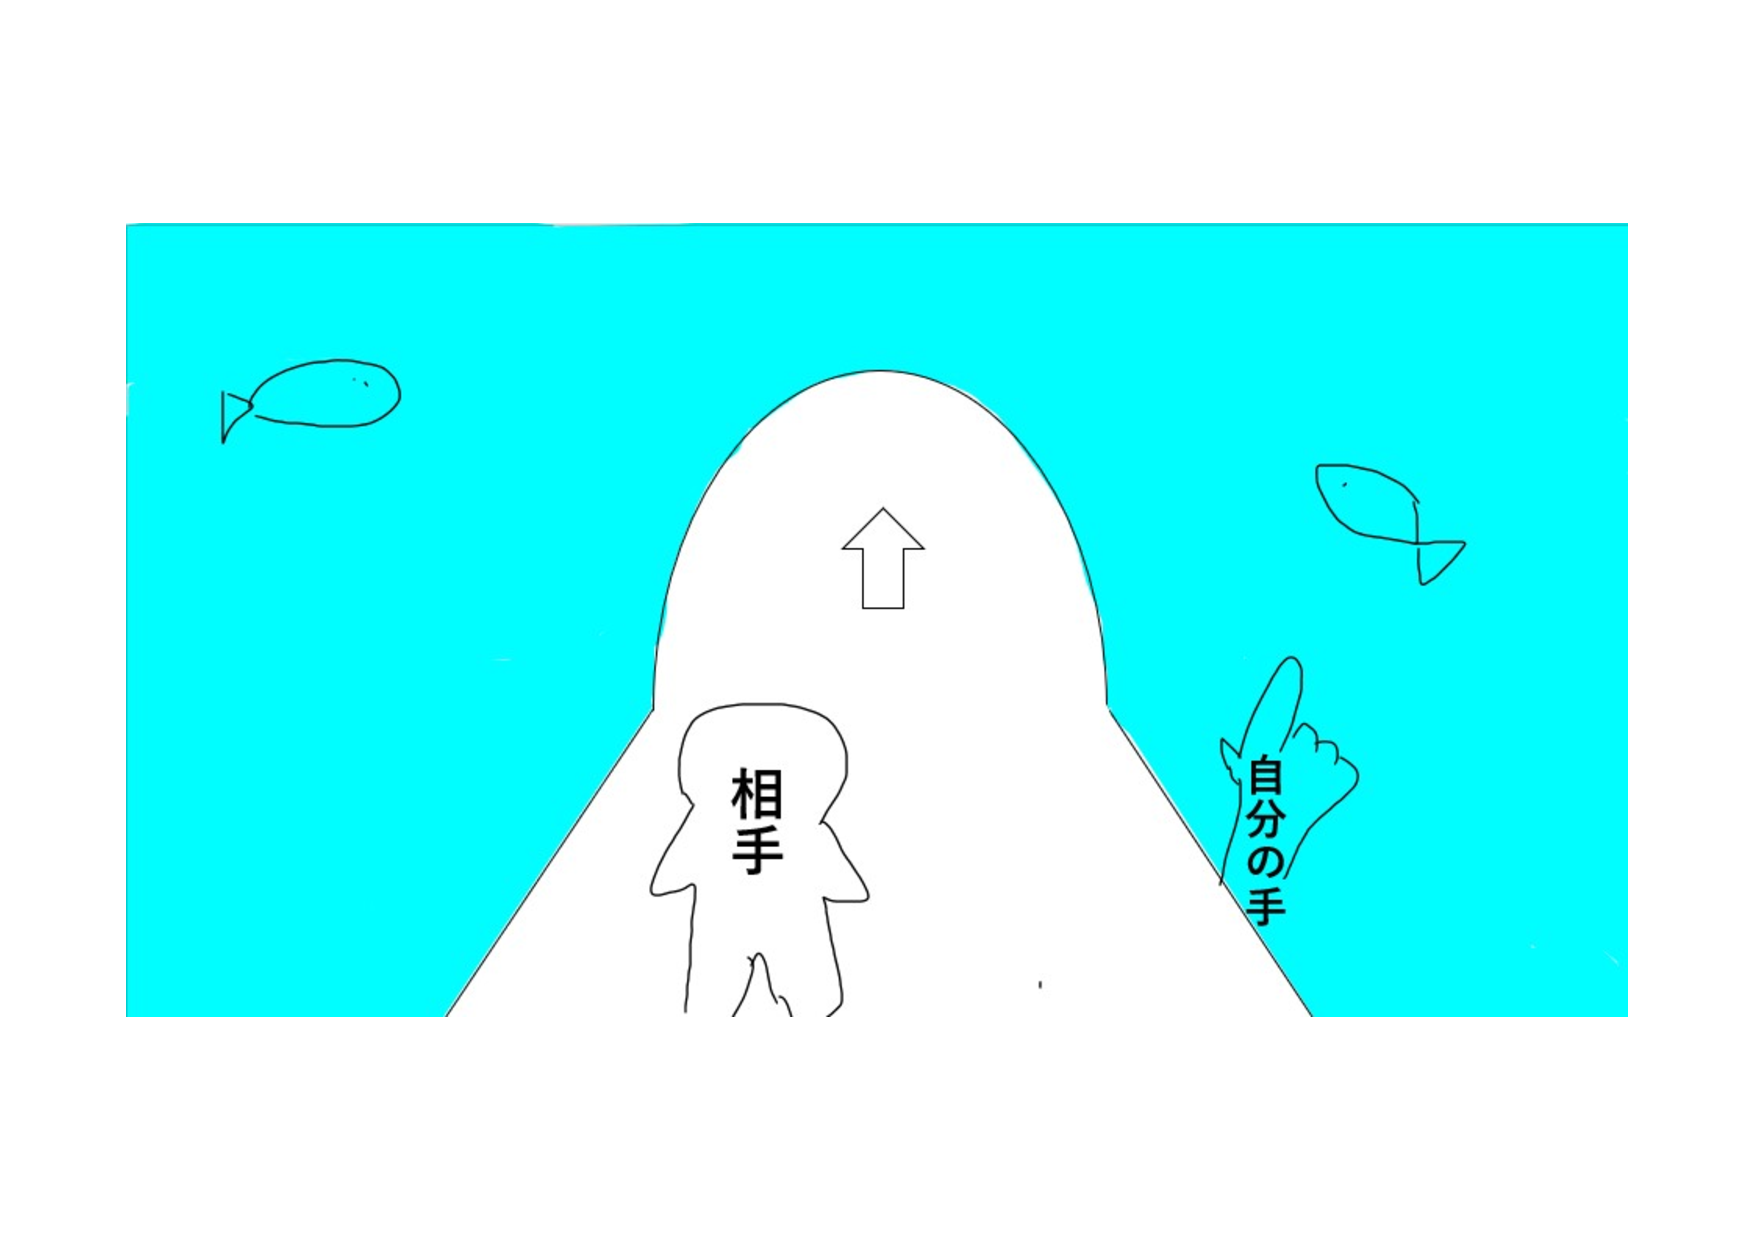
\includegraphics[width=150mm]{irasuto.jpg}
\end{center}
 \caption{VRアプリの仮定イラスト}
 \label{fig:イラスト}
\end{figure}

% VRChatとの違い

今現在流行しているVRchatとの相違点は,VRchatは自由度が高く出来ることが多いためデート初心者にとっては何処に行けば良いのか,何をしたら良いのかの選択肢が広く計画を立てるのが困難である.
本研究のVRデートアプリでは,初デートへのハードルを下げることを考えて40分から1時間程度の時間制限を設けアトラクション式の視点移動型のVRを考えている.
VRchatと比較した際にデートに特化しており気楽にデートをすることができる.

このアプリケーションの使用前と使用後でそれぞれアンケートを行いユーザーが交際に対して前向きになることができたのか,デートへの壁がなくなったのかを調査する.

現時点で行ったことは類似アプリケーションの確認である.本研究テーマと同じアプリのものがあるのかを確認したが現在のところ同じ目的を持ったアプリケーションは存在していない.




\section{今後の予定}
4年生の内にデートができ,アプリ内で会話が行えるようなシステム開発を行う.
大学院1年生では,アンケート項目を決めるための予備調査やアプリケーションを使用してもらい簡易的な実験を行う.
大学院2年生では,実験を重ね,調査を行い,論文を作成し,学会で発表することを視野に入れている.

\begin{thebibliography}{99}
\bibitem{sasaki2012} 佐々木 尚之: ``不確実な時代の結婚-JGSSライフコース調査による潜在的稼得力の影響の検証'', 「家族社会学研究」,第24号,pp152-164(2012)
\bibitem{naikakufu2019} 内閣府: ``少子化対策の現状'', \url{https://www8.cao.go.jp/shoushi/shoushika/whitepaper/measures/w-2016/28webhonpen/html/b1_s1-1-3.html}, 2019/3/26参照
\bibitem{doukou}国立社会保障・人口問題研究所:``第15回出生動向基本調査'',
\url{https://www.ipss.go.jp/ps-doukou/j/doukou15/NFS15_report3.pdf},2022/3/14参照
\bibitem{cancan}CanCan.jp:``実は「今、恋人がいる」人は3割だけ。新成人618人に聞いた恋愛・結婚観'',
\url{https://cancam.jp/archives/1078613},2022/1/8参照
\bibitem{prtimes}PRTIMES:``マッチングアプリは怖い?危ない目に合った?初めて会うまでの期間は!?徹底調査'',
\url{https://prtimes.jp/main/html/rd/p/000000016.000059676.html},2021/10/4参照
\bibitem{yoshimura2020} 古村 健太郎: ``成人のマッチングアプリ利用の背景-成人のマッチングアプリ利用に関する研究'', 「日本心理学会大会発表論文」,第84号,pc-006(2020)

\end{thebibliography}

\end{document}
